\documentclass[border=10pt]{standalone}
\usepackage{tikz}

\begin{document}
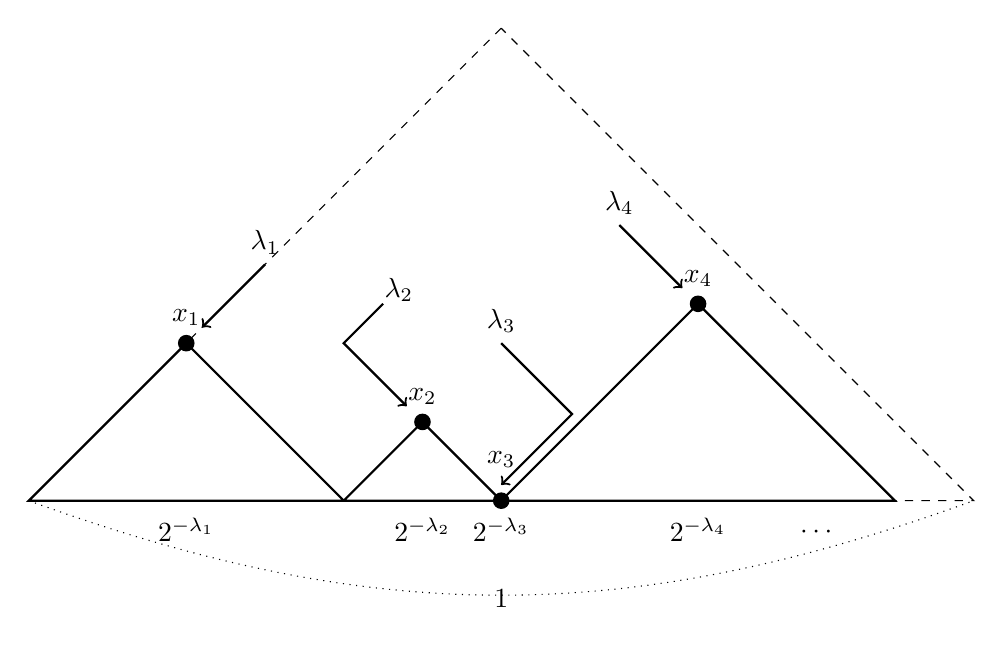
\begin{tikzpicture}[scale=1]

    \draw[dashed] (0,6) -- (-6,0) -- (6,0) -- (0,6);

    \fill (-4,2) circle (3pt) node[above] at (-4,2.1) {$x_1$};
    \draw[thick] (-4,2) -- (-6,0) -- (-2,0) -- (-4,2);
    \draw[thick,->] (-3,3) -- (-3.8,2.2) node[above] at (-3,3) {$\lambda_1$};
    \node[below] at (-4,-0.1) {$2^{-\lambda_1}$};

    \fill (-1,1) circle (3pt) node[above] at (-1,1.1) {$x_2$};
    \draw[thick] (-1,1) -- (-2,0) -- (0,0) -- (-1,1);
    \draw[thick,->] (-1.5,2.5) -- (-2,2) -- (-1.2,1.2) node[above] at (-1.3,2.4) {$\lambda_2$};
    \node[below] at (-1,-0.1) {$2^{-\lambda_2}$};

    \fill (0,0) circle (3pt) node[above] at (0,0.3) {$x_3$};
    \draw[thick,->] (0,2) -- (0.9,1.1) -- (0,0.2) node[above] at (0,2) {$\lambda_3$};
    \node[below] at (0,-0.1) {$2^{-\lambda_3}$};

    \fill (2.5,2.5) circle (3pt) node[above] at (2.5,2.6) {$x_4$};
    \draw[thick] (2.5,2.5) -- (0,0) -- (5,0) -- (2.5,2.5);
    \draw[thick,->] (1.5,3.5) -- (2.3,2.7) node[above] at (1.5,3.5) {$\lambda_4$};
    \node[below] at (2.5,-0.1) {$2^{-\lambda_4}$};
    \node[below] at (4,-0.2) {$\cdots$};

    \draw[dotted,-] (-6,0) to[out=-20,in=200] (6,0);
    \node[below] at (0,-1) {$1$};

\end{tikzpicture}
\end{document}